% Chapter X

\chapter{Inflammation dans la mucoviscidose} % Chapter title


\label{ch:02-04} % For referencing the chapter elsewhere, use \autoref{ch:name} 

%----------------------------------------------------------------------------------------

% \section{}

\section{Inflammation généralité}
Nous vivons dans un monde inondé d’agresseurs trop petit pour être détectés à l’œil nu, et aucun vertébré ne pourrait résister longtemps à leur attaque s’il n’était protégé. Nous survivons parce que nous avons acquis au cours de l’évolution divers mécanismes de défenses très efficaces contre ces attaques permanente et il importe de garder à l’esprit que bien qu’efficace ils sont loin d’être parfait. 
Un vertébré se défend contre une infection à l’instar d’un chevalier qui défendait les cités médiévales. Les « remparts et les fossés » rende l’invasion difficile, les « sentinelles » interpelles tout ce qui erre dans les environ et font appel aux « patrouilles » si un inconnu ne peut prouver son innocence :
\begin{itemize}
\item Les remparts et fossés : la peau, couche externe du corps des vertébré, est la première barrière que doivent franchir les microbes. Les muqueuses des tractus respiratoire, digestif et urogénital font également partie de l’enceinte protectrice.
\item Les sentinelles : Appartenant au système immunitaire certaines de ces cellules sont particulièrement agressives et tuent (par phagocytose) tous éléments reconnus comme étrangers, ou les virus afin qu’ils soient reconnus et éliminés par les patrouilles. Les cellules sentinelles (ou résidantes des tissus) comprend les phagocytes mononucléés résidents (cellules dendritiques et macrophages) ainsi que les mastocytes. Si cette première ligne de défense des sentinelles était franchie, l’organisme réagirait en organisant une contre-attaque cellulaire capable de tuer l’élément étranger. Ce moyen de défense entre en action très rapidement après le début de l’infection. Elles sont activées en contact avec les éléments étrangers, en réponse elles vont libérer des médiateurs de l’inflammation notamment des cytokines pro-inflammatoires et de l’histamine, un vasodilatateur qui va favoriser le recrutement des « patrouilles » dans les tissus.
\item Les patrouilles : Les cellules qui patrouillent via le sang dans l’ensemble de l’organisme sont les lymphocytes T et B, les cellules NK, les monocytes qui vont maturer en macrophages en gagnant le tissu où ils seront qualifiés de résident, et la famille des granulocytes dont l’activité s’exerce au niveau des tissus et qui comprend les polynucléaires basophiles, éosinophiles et neutrophiles. Ces cellules comptent parmi les leucocytes les plus nombreux dans la circulation périphérique. Ils ont un noyau multilobé et de nombreuses granules dans leur cytoplasme, entre les divers types de granulocytes d’importantes différences fonctionnelles existent. 
\end{itemize}
Patrouilles et sentinelles forment l’inflammation et constitue l’un des mécanismes les plus importants des défenses de l’organisme. Il existe de multiples causes à l’origine de l'inflammation, comme les agressions de types physiques (traumatisme, chaleur/ froid, radiations) ou chimiques (agents caustiques, toxines, venins).il y a aussi l’infection par des micro-organismes comme les bactéries, virus, parasites et champignons ou une agression dys-immunitaire (anomalie de la réponse immunitaire, allergies …) qui sont capable de déclencher une inflammation. Dans tous les cas l’agent pathogène peut être soit endogène ou exogène, plusieurs causes peuvent être associées dans le déclenchement de l’inflammation et pour un même agent pathogène on peut avoir des réactions inflammatoires différentes selon l’hôte et l’état de ses défenses immunitaire. (Figure \ref{inflammation})
\begin{center}
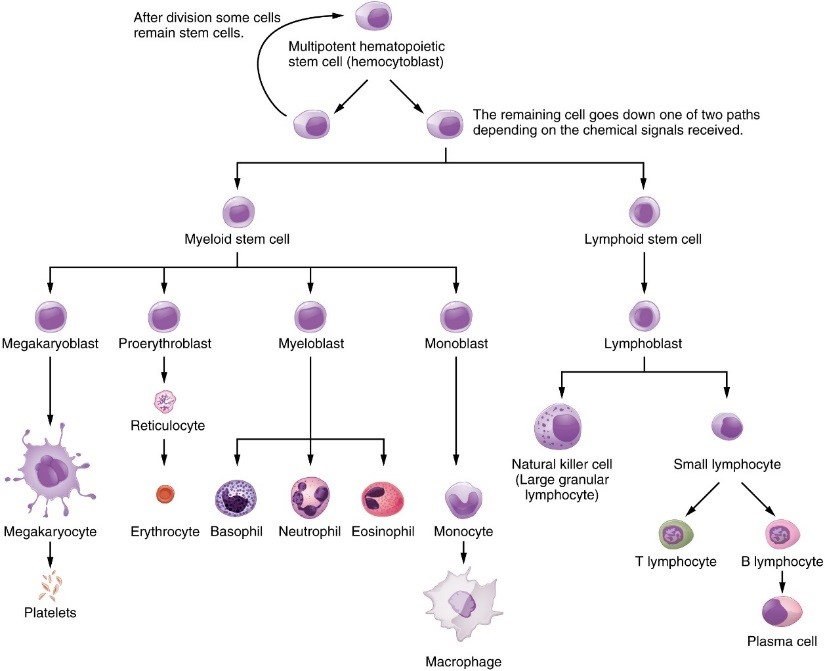
\includegraphics[scale=1]{gfx/inflammation.jpg} 
\captionof{figure}{Cellules de l'inflammation}
       \label{inflammation}
\end{center}

La réaction inflammatoire ou inflammation est définie comme la réponse locale à toutes sortes d’agression de tissus vascularisé et vivant. Habituellement bénéfique pour l’organisme, ce processus a pour but de réparer les lésions et d’éliminer l’agent pathogène, mais peut conduire dans certain cas à une inflammation néfaste pour l’organisme en raison de l’agressivité ou de la persistance de cet agent. D’autres causes, comme des anomalies dans la régulation du processus inflammatoire ou lorsque la quantité ou la qualité des éléments intervenant dans l’inflammation sont altérés peuvent aussi conduire à une inflammation néfaste. Ce qui est le cas dans la mucoviscidose qui est caractérisée par des atteintes pulmonaires progressives graves qui sont la cause principale de mortalité et morbidité chez les patients.

		\section{Cas de la mucoviscidose}
Au cours de ces 30 dernières années de nombreuse recherche ont été effectué concernant l’origine de cette réponse inflammatoire qui commence très tôt, qui persiste, qui deviens excessive à la suite d’une infection et qui se révèle le plus souvent inefficace dans la mucoviscidose (Nixon et al. 2002; Khan et al. 1995; Balough et al. 1995; Chen and Nuñez 2010; Pillarisetti et al. 2011)\cite{nixon_early_2002}\cite{khan_early_1995}\cite{balough_relationship_1995}\cite{chen_sterile_2010}\cite{pillarisetti_infection_2011}. La libération d’élastase et d’autre protéinase par les neutrophiles est considérée comme l’élément clé contribuant aux dommages pulmonaire associé à la réponse inflammatoire (Armstrong et al. 1995)\cite{armstrong_lower_1995}. Chez les patients atteints de mucoviscidose l’activité de l’élastase et des autres protéines est très élevée comparé à ceux des personnes non atteints (Downey, Bell, and Elborn 2009)\cite{downey_neutrophils_2009}. On constate aussi des changements structurels aux niveaux des voies aériennes et un encombrement des bronchioles dû à l’épais mucus produit par les glandes sécrétrices hypertrophiées(Hays and Fahy 2006)\cite{hays_characterizing_2006}. 
Parmi les pathogènes qui colonise les voies aérienne des patients atteint de mucoviscidose les plus fréquemment retrouvés sont Pseudomonas Aeruginosa, Staphylococcus Aureus et Haemophilus Influenzae (Saiman 2004)\cite{saiman_microbiology_2004}. Souvent la réponse des patients à l’infection est excessive. Une bronchectasie finie par se développer à cause d’une obstruction des voies respiratoire et des infections bactériennes constantes liées à une réponse inflammatoire exacerbée. Depuis peu le précepte considérant que l’infection initie l’inflammation est remis en question. La mutation CFTR étant elle-même capable d’induire directement l’inflammation en absence d’infection (Rao and Grigg 2006)\cite{rao_new_2006}. Tout ceci montre l’importance de l’inflammation dans la mucoviscidose. 

			\subsection{Mécanismes cellulaire des réactions inflammatoires }
			 \subsubsection{Macrophages}
Dans la mucoviscidose a été observé un défaut dans plusieurs fonctions des macrophages (Hubeau, Puchelle, and Gaillard 2001)\cite{hubeau_distinct_2001}. Ils présentent une diminution de leurs capacités de clearance des cellules apoptotique(Vandivier, Fadok, Hoffmann, et al. 2002; Vandivier, Fadok, Ogden, et al. 2002)\cite{vandivier_elastase-mediated_2002}\cite{vandivier_impaired_2002}, de la production de cytokines(Bonfield et al. 1995)\cite{bonfield_normal_1995} et de la phagocytose(Knight et al. 1997; Di et al. 2006)\cite{knight_defective_1997}\cite{di_cftr_2006}. Il semble aussi qu’il y a une dérégulation dans le recrutement de macrophages et de leurs fonctions bien avant leurs stimulations par l’infection(Starner et al. 2003)\cite{starner_ccl20_2003}. 

			\subsubsection{Neutrophiles }
Les fonctions des neutrophiles sont la défense de l’hôte, la phagocytose et la destruction de pathogènes invasifs(Hampton, Kettle, and Winterbourn 1998)\cite{hampton_inside_1998}. En réponse à une infection les neutrophiles génèrent des espèces réactives de l’oxygène (ROS) via la NADPH oxydase et secrète des protéines granulaires anti microbiennes comprenant entre autre l’élastase, la collagénase, les cathepsines et la myeloperoxidase afin de protéger l’organisme. De l’ADN peut être libéré par les neutrophiles pour former des NETS (neutrophil extracellular traps) qui vont piéger les bactéries afin de les éliminer(Brinkmann et al. 2004; Brinkmann and Zychlinsky 2007)\cite{brinkmann_neutrophil_2004}\cite{brinkmann_beneficial_2007}. Si cette réponse est non contrôlée, il peut en résulter des dommages aux tissues excessifs graves et qui représentent la majorité des dommages pulmonaire observées chez les patients atteint de mucoviscidose. Sous hypoxique, condition caractéristique d’un mucus mucoviscidosique, les neutrophiles vivent plus longtemps, augmentant ainsi leurs potentiels d’endommagement du poumon(Walmsley et al. 2005)\cite{walmsley_hypoxia-induced_2005}. Chez des enfants et fœtus atteint de mucoviscidose on dénombre une quantité important de neutrophiles au niveau des voies respiratoires qui augmente au fur et à mesure que la maladie progresse(Rosenfeld et al. 2001; Muhlebach and Noah 2002)\cite{rosenfeld_early_2001}\cite{muhlebach_endotoxin_2002}. De plus il a été montre qu’il y a un défaut dans le contrôle de la réponse inflammatoire à la suite d’une stimulation qui est associé à une inhabilité à phagocyter et à débarrasser les poumons des bactéries(Armstrong et al. 1995)\cite{armstrong_lower_1995}. Un nombre certains d’études on montrés une multitude de différences entre les neutrophiles issus de patients atteint de mucoviscidose et ceux de patients sains notamment une augmentation de la production de ROS(Graff, Schram-Doumont, and Szpirer 1991)\cite{graff_defective_1991}, une augmentation de la dé-granulation(Koller, Urbanek, and Götz 1995)\cite{koller_increased_1995}, une augmentation dans l’activité protéolytique avec une augmentation de la libération d’élastase(Gaggar et al. 2007; Brockbank et al. 2005)\cite{gaggar_matrix_2007}\cite{brockbank_effect_2005} et de Métalloprotéinase matricielle (MMP)(Ratjen et al. 2002; Sagel, Kapsner, and Osberg 2005; Gaggar et al. 2007)\cite{ratjen_matrix_2002}\cite{sagel_induced_2005}\cite{gaggar_matrix_2007}, une augmentation de l’apoptose(Watt et al. 2005; Vandivier, Fadok, Ogden, et al. 2002)\cite{watt_neutrophil_2005}\cite{vandivier_impaired_2002}, une diminution dans l’activité antimicrobienne(Moraes et al. 2006) \cite{moraes_abnormalities_2006}et une dérégulation dans la production de cytokines(Corvol et al. 2003)\cite{corvol_distinct_2003}.

			\subsubsection{Epithélium}
L’épithélium pulmonaire participe activement à l’immunité innée et orchestre les réponses inflammatoires. L’interaction des pathogènes avec l’épithélium des voies aérienne est une étape indispensable à l’activation des mécanismes de défense impliquant les neutrophiles et les macrophages. La stimulation de l’épithélium par les pathogènes se fait via l’activation des toll-like récepteurs (TRL)(Machen 2006; Muir et al. 2004)\cite{machen_innate_2006}\cite{muir_toll-like_2004} par différents ligand (lipopeptides, peptidoglycane, acide lipotéichoïque, fragment CXCR1) et l’activation des voies de transcription AP-1 et NF-$\kappa$B (Moskwa et al. 2007)\cite{moskwa_novel_2007} résultant à la production de cytokine pro inflammatoire responsable du recrutement des leucocytes et monocytes(Zhang et al. 2005)\cite{zhang_human_2005}. 
En temps normal l’induction d’ARN messager de cytokine pro-inflammatoire comme entre autre IL-8, GRO-$\alpha$, MIP-3 diminue après une exposition chronique aux produits bactériens. Par contre la production de cytokine suite à une infection par Pseudomonas Aeruginosa ne baisse pas nécessairement chez les patients atteints de mucoviscidose suggérant une inflammation soutenue des voies aérienne(Nichols, Chmiel, and Berger 2008)\cite{nichols_chronic_2008}.
Plusieurs défauts ont été proposés à ce jour en relation avec la fonction épithéliale dans la réponse inné, notamment un défaut dans le contrôle de l’équilibre redox qui est sans aucun doute le plus marquant. En effet une diminution de la fonction CFTR a été montrée comme associée à une diminution du transport de la GSH dans la lumière des voies respiratoires(Gao et al. 1999; Velsor, van Heeckeren, and Day 2001)\cite{gao_abnormal_1999}\cite{velsor_antioxidant_2001}. Il a été montré aussi qu’un défaut de CFTR entraine un effet sur l’expression des gènes associé à la balance redox(Xu et al. 2006)\cite{xu_functional_2006} et présente une augmentation du stress oxydatif dans les voies respiratoires de jeunes patients atteint de mucoviscidose(Kettle et al. 2004)\cite{kettle_myeloperoxidase_2004}. De plus un défaut de l’activité oxydative des cellules de l’épithélium a été montré comme associé à un défaut dans l’activité bactéricide des cellules(Moskwa et al. 2007)\cite{moskwa_novel_2007}. Tout ceci porte à croire qu’un défaut dans le contrôle de l’équilibre redox semble être à l’origine des problèmes inflammatoires observés chez les patients atteints de mucoviscidose.


%------------------------------------------------

% \subsection{Subsection Title}

% Content